\section{Preliminary Resutls and Future Work}

\begin{figure}[!h]
  \centering
  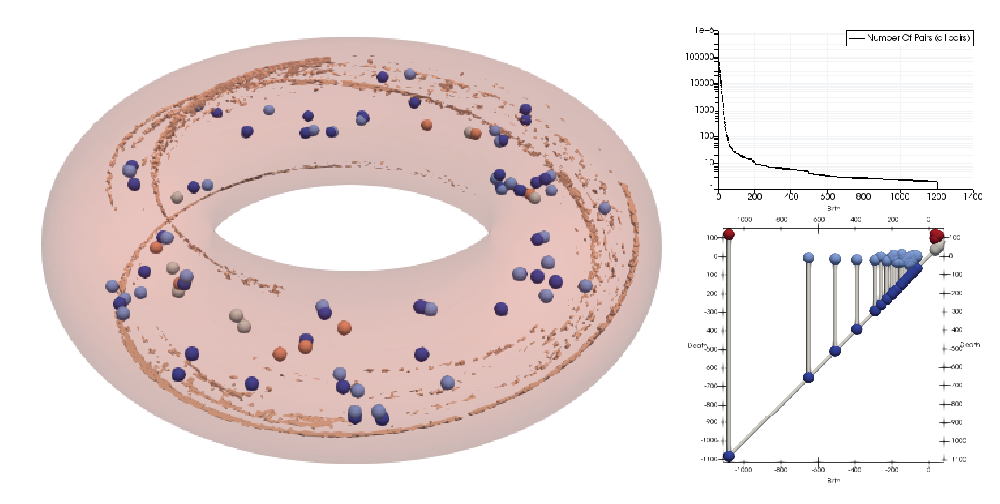
\includegraphics[width=\linewidth]{Figs/simplification3D}
  \caption{Topology simplification of a 3D XGC simulation dataset.}
  \label{fig:results}
\end{figure}


%\begin{figure}[!htb]
%  \centering
%  \includegraphics[width=\linewidth]{Figs/results}
%  \caption{Preliminary results: (a) the 2D triangular mesh; (b) critical points extracted in a slice.}
%  \label{fig:results}
%\end{figure}

Figure~\ref{fig:results} presents our preliminary results.  We are already able to extract critical points in individual slices.  We will associate these points across different slices and timesteps for the next milestones.  We are also going to incorporate the RPCA into the workflow to simplify the input data.  We would also like to have discussions with fusion scientists to evaluate our approach.  


Contour tree instead of Reeb graphs.  